%!TEX root = ../Report.tex

In this chapter, we will discuss the design of the system created to investigate this problem, and detail how such a system could be extended for the future.



\section{System description}

The ideas described in the background section are combined to produce a skeleton programming library which utilizes plasticity and contention aware scheduling. To keep it simple, we build the system incrementally, starting with a single parallel pattern, later adding plasticity and contention aware scheduling. 



\subsection{Skeleton Foundation}
\label{section:design_skeleton_foundation}

As discussed in the background section, one of the key ideas behind the project is that of skeleton programming, using predefined patterns to aid the programmer. Possibly the most common skeleton is map, which is a skeleton that takes a function, an array of data, and applies the function to each member of the array. The map operation itself is inherently parallelizable, since each `task' (processing one element of the input array) is independent, so we can simply assign different chunks of the input array to different threads. This is called an ``embarrassingly parallel'' problem. 

Other such patterns include map-array, reduce, and scan. These are all implemented in SkePU with a corresponding skeleton (as described in section \ref{section:background_what_is_skeleton_programming}.) In our case, we will focus on the map-array pattern, with further patterns left for possible future work. Map-array is similar to the map pattern in that it applies a given user function to each element in a list, however map-array also allows the function to access a user provided array. A diagram to better explain this is given in figure \ref{fig:skepu_skeletons}.

Map-array was chosen as the focus of the project as the map pattern is likely the most well known pattern and certainly one of the most useful, and map-array provides further functionality on top of this. It also provides a good basis for developing further patterns, and allows for the testing of more complex situations, which will be covered in chapters \ref{chapter:experimental_methodology_and_program} and \ref{chapter:future_work_and_conclusions} of this report.



\begin{figure}
	\centering
	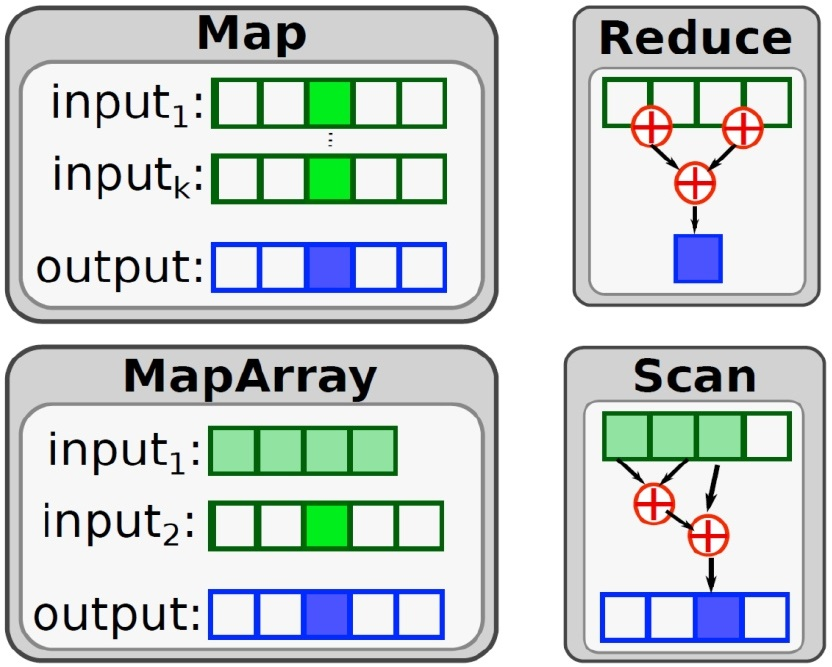
\includegraphics[width=0.7\textwidth]{graphics/skepu_skeletons.jpg}
	\caption{Taken from SkePU documentation: Examples of patterns}
	\label{fig:skepu_skeletons}
\end{figure}



\subsection{Adding Plasticity}
\label{subsection:design_adding_plasticity}

To implement plasticity, we add the ability to vary three key aspects of the implementation of a single instance of the map-array skeleton:

\begin{itemize}
	\item Thread count - The number of threads we split the tasks between
	\item Thread pinnings - The particular CPU core each thread runs on
	\item Schedule - How to divide tasks between threads
\end{itemize}

The thread count and pinnings are self explanatory. The schedule however requires some explanation.

The most basic method to divide the tasks is to give an equal amount to each thread. This is fine if the complexity of the tasks is uniform, but if it is biased (e.g. tasks in the first portion of the array are more complex than the rest), the amount of computation to be done by each thread is imbalanced. This is because we have idle cores during computation, since the threads with more work will still be computing once the others have finished. This downtime is a wasted resource in a multi-threaded execution. However, if we allocate the tasks differently, we can obtain better performance, as illustrated in figure \ref{fig:schedule_optimization}, where the improved schedule runs twice as fast as the simple one.

So load balancing a workload is critical to performance in such a multi-threaded application. However, optimizing the task distribution in this manner is a non trivial problem, and it depends upon the computation to be done as well as the number of threads and other resources available at runtime.

A solution to this problem is to provide many different task distributions, and let the user pick or the machine select which distribution to use. OpenMP documentation calls these schedules, and some examples of these are:

\begin{itemize}
	\item Static - An equal number of tasks allocated to all threads
	\item Dynamic individual - Each thread retrieves one task at a time, and once completed, it goes back for more
	\item Dynamic chunks - Each thread retrieves N tasks at a time, and once completed, it goes back for more
	\item Tapered - Each thread starts by retrieving N tasks at a time, and as the computation continues, it retrieves fewer and fewer
\end{itemize}

Thread count and schedule were chosen as they seem the most critical to performance, and thread pinnings was added as this is was investigated in the LIRA paper \cite{lira} as a factor contention aware scheduling could exploit.

Once we have added plasticity, we can experiment with the specifics of an implementation, and see how they affect the performance of the system. This would be the use case of utilizing our library with no other program running, (So no contention aware scheduling), and we can explore how we can adapt the program using plasticity at runtime in this case. We may be able to improve performance even under these conditions, depending upon the configuration of the machine (e.g., are there more CPU cores available) and the problem (e.g. do we have many small tasks or few large tasks.) 



\begin{figure}[!]
	\centering
	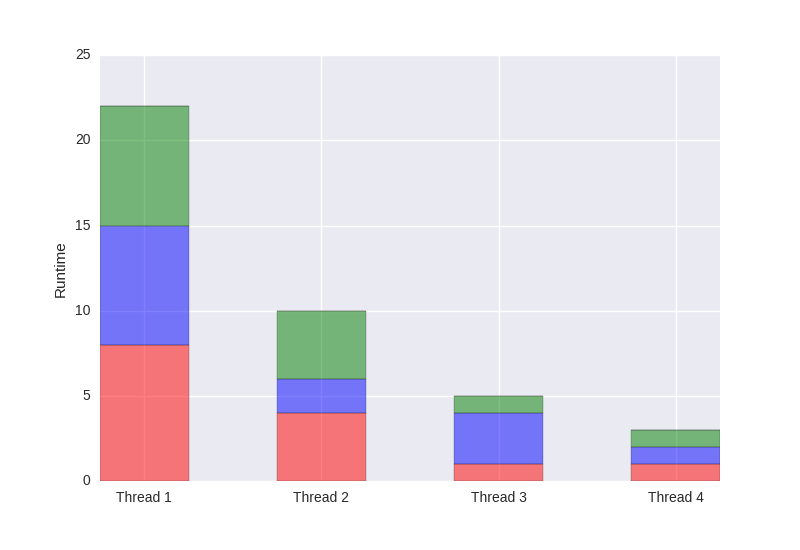
\includegraphics[width=0.9\textwidth]{graphics/unoptimized_schedule.png}
	\caption{A worst case scenario of a static schedule assigning each thread an equal number of tasks. Suppose we have a set of twelve independent tasks with the following set of execution times (These would be unknown to the scheduler): \{10, 6, 4, 4, 2, 2, 2, 2, 1, 1, 1, 1\}. With four threads, a simple division of tasks would be three tasks each distributed in order. This figure illustrates this distribution of work. Note that the total execution time is 20 time units.}
	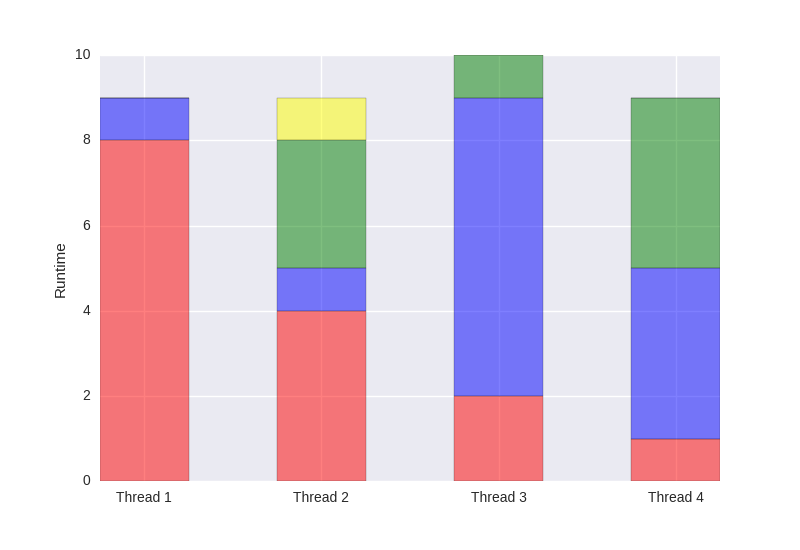
\includegraphics[width=0.9\textwidth]{graphics/optimized_schedule.png}
	\caption{An optimized version of the previous schedule. Here we have the same set of tasks, but we have a better distribution of work, so the total execution time is 10 time units.}
	\label{fig:schedule_optimization}
\end{figure}



\subsection{Contention Aware Scheduling}
\label{subsection:design_contention_aware_scheduling}

To add contention aware scheduling, we need multiple applications using our library to be able to collaborate, and adapt their behaviour accordingly. To do this, we use a separate controller application, with which all instances of our program can communicate. This provides a single known point of contact, and a designated thread for computing program parameters with respect to all aspects of the system.

Once our programs can communicate, and we can control each aspect of them, we can implement contention aware scheduling. In this phase of the project, we simply program a set of predefined actions for the controller to take, in order to manually control what each implementation does, as we are only investigating if this approach seems promising. We leave implementing some algorithm for automatic parameter tuning for future work.

A diagram showing the high level communication model is given in figure \ref{fig:communication_structure}. This is expanded upon in section \ref{section:implementation_contention_aware_scheduling}, showing specifics about the implementation.

With contention aware scheduling, we can experiment with multiple programs running on a system at once. An example of how contention aware scheduling can be enhanced with plastic programming is given in figure \ref{fig:plastic_contention_aware_scheduling}.



\begin{figure}
	\centering
	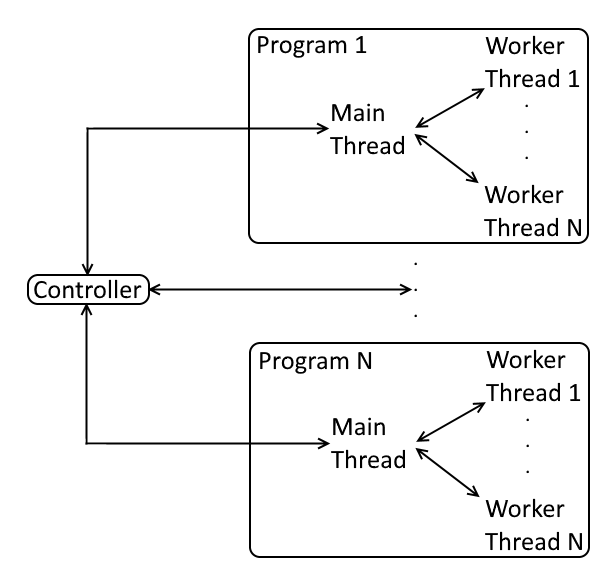
\includegraphics[width=\textwidth]{graphics/communication_structure.png}
	\caption{High level communication model of the system, with an arbitrary number of programs, with an arbitrary number of threads. Two way communication occurs between the controller and each main thread, and then between each main thread and it's worker threads.}
	\label{fig:communication_structure}
\end{figure}

\begin{figure}
	\centering
	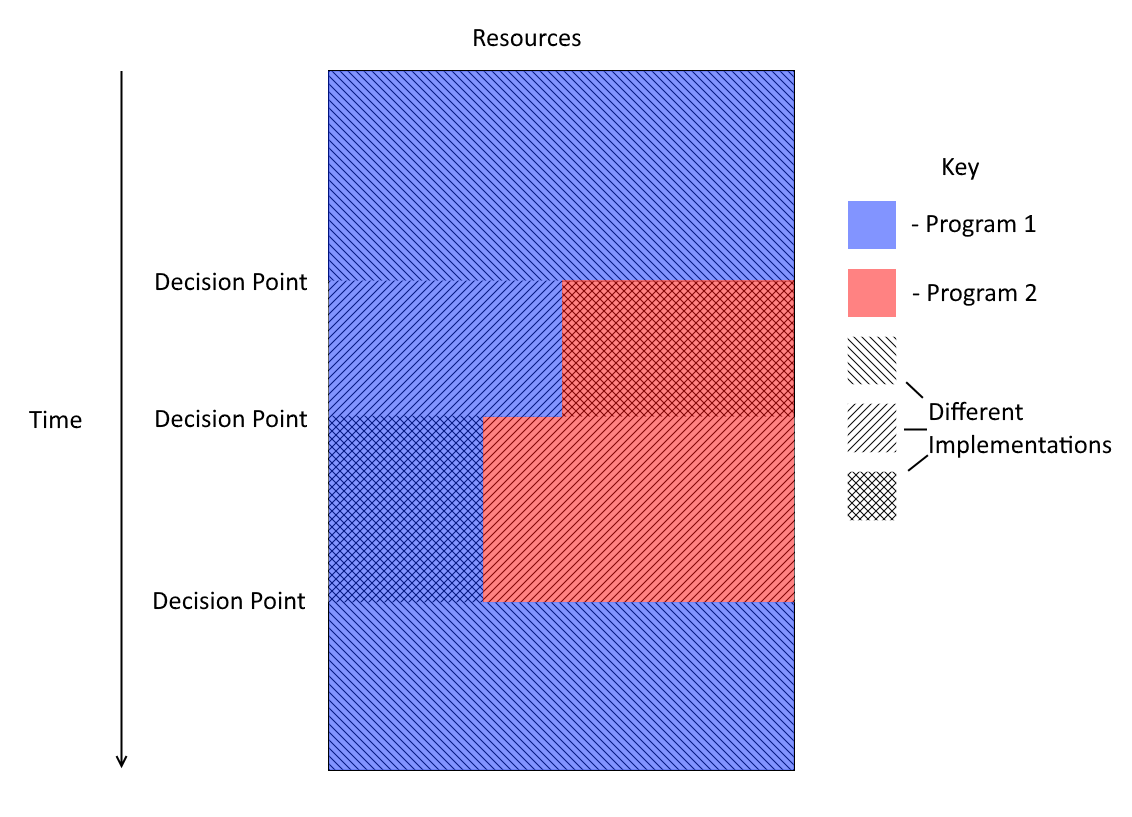
\includegraphics[width=\textwidth]{graphics/plastic_contention_aware_scheduling.png}
	\caption{An example of how contention aware scheduling can be enhanced with plastic programming. We have two programs, represented by different colours. As time progresses, we see that when program 2 launches, we have a decision point. Here, the system decides how many resources to give each program and what implementation they should use, according to what is optimal (In this project, we do this manually.) \\ \\ Moving further in time, we have another decision point. This one is triggered by some other change in the machine, which means the optimal configuration has changed. So the system updates the configuration of each program, and continues. \\ \\ Program 2 then terminates, triggering another decision point, and the system again updates the configuration.}
	\label{fig:plastic_contention_aware_scheduling}
\end{figure}



\subsection{Evaluation}

To properly evaluate the outcome of this project, we need some way of testing the libraries performance. To this end, we implemented a synthetic program which calls the skeleton with an artificial workload, collecting and recording metrics detailing the libraries performance with different parameters.  

We also need points of comparison in terms of performance. So, in addition to our synthetic program, we also implement an equivalent sequential and an OpenMP version, in which we can vary similar parameters and produce comparable statistics. 

The detailed experimental program will be discussed in chapter \ref{chapter:experimental_methodology_and_program}.